\documentclass[11pt]{article}
\usepackage{fullpage}
\usepackage{amsmath,amsfonts,amsthm,amssymb}
\usepackage{url}
\usepackage{graphicx}
\usepackage{caption} 
\usepackage{algpseudocode}
\usepackage{bbm}
\usepackage{float}
\usepackage{framed}
\usepackage{enumerate}
\usepackage{color}
\usepackage[colorlinks=true, linkcolor=red, urlcolor=blue, citecolor=blue]{hyperref}
\usepackage{listings}

\DeclareMathOperator*{\E}{\mathbb{E}}
\DeclareMathOperator*{\pr}{\mathbb{P}}
\DeclareMathOperator*{\Var}{\textrm{Var}}
\DeclareMathOperator*{\I}{\mathbb{I}}
\DeclareMathOperator*{\R}{\mathbb{R}}

\renewcommand{\lstlistingname}{Algorithm}% Listing -> Algorithm
\lstset{%
%    basicstyle=\small\ttfamily,
    escapechar=~,
    frame=single,
    keywordstyle=\bfseries,
    keywords={input,output,for,return,if,in,then,do},
    mathescape=true,
    morecomment=[l][\color{blue}]{\#},
    numbers=left,
    xleftmargin=.04\textwidth
}

\topmargin 0pt
\advance \topmargin by -\headheight
\advance \topmargin by -\headsep
\textheight 8.9in
\oddsidemargin 0pt
\evensidemargin \oddsidemargin
\marginparwidth 0.5in
\textwidth 6.5in

\parindent 0in
\parskip 1.5ex

\newcommand{\homework}[2]{
	\noindent
	\begin{center}
		\framebox{
			\vbox{
				\hbox to 6.50in { {\bf NYU CSCI-GA.2566-001: 
				Foundations of Machine Learning 
				} \hfill Fall 2020 }
				\vspace{4mm}
				\hbox to 6.50in { {\Large \hfill Homework #1  \hfill} }
				\vspace{2mm}
				\hbox to 6.50in { {Name: #2 \hfill} }
			}
		}
	\end{center}
	\vspace*{4mm}
}

\newcommand{\braket}[2]{\langle #1, #2\rangle}
\newcommand{\norm}[1]{||#1||_2}

\begin{document}
	
%\homework{1}{R. Teal Witter}
%% chktex-file 46
% chktex-file 3

\section*{A. Consistent hypotheses}
\medskip

Let $Z$ be a finite set of $m$ labeled points.
Suppose we have a PAC-learning algorithm $A$.
Then
for all concepts $c$ in the concept class $C$,
all $\epsilon > 0$, all $\delta > 0$, and all distributions
$D$ over $Z$,
\begin{align}
    \pr_{S \sim D^m}[R(h_S)\leq \epsilon]
    \geq 1 - \delta
    \nonumber
\end{align}
for hypothesis set $h_S$ which depends
on sample $S$.
In other words,
with probability $1-\delta$ for $S\sim D^m$,
\begin{align}\label{eq:rhs}
    R(h_S) = \pr_{x\in D}[h_S(x)\neq c(x)] \leq \epsilon
\end{align}
from the definition of $R(h)$ on page 6 of Lecture 02.

We want to show that we can find a hypothesis
$h \in H$ that is consistent with $Z$ with
probability at least $1-\delta'$ for $\delta'>0$.

Fix $m$ the size of $Z$ and $\delta' >0$.
Now choose $D$ to be the uniform
distribution, $\epsilon=\delta'/2m$,
and $\delta=\delta'/2$.
We train $A$ with these parameters
on a sample $S$ drawn from $D^m$.

We now argue that hypothesis $h_S$
on $S$ is consistent with $Z$ with probability
at least $1-\delta'$.

Observe that the probability $h_S$
is consistent with $Z$ is the complement
of the probability that $h_S$ makes an
error on some element $x$ in $Z$.
That is,
\begin{align}
    \pr(R(h_S) = 0) &= 1
    - \pr(h_S(x) \neq c(x)
    \textrm{ for some } x \in Z)
    \label{eq:first} \\
    &\geq 1 - m \pr(h_S(x) \neq c(x))
    \label{eq:second} \\
    & \geq 1- m \frac{\delta'}{2m}
    = 1 - \frac{\delta'}{2}
    \label{eq:third}
\end{align}
where \autoref{eq:second} follows
from \autoref{eq:first} by the Union Bound
and \autoref{eq:third} follows from
\autoref{eq:second} by \autoref{eq:rhs}.

Therefore $h_S$ is consistent with $Z$
with probability $1-\delta'/2$ times
the probability \autoref{eq:rhs} holds
which is also $1-\delta'/2$.
That total probability is
\begin{align}
    1-2\frac{\delta'}{2} + \frac{\delta'^2}{4}
    \geq 1-\delta'
    \nonumber
\end{align}
as required.

Clearly the time complexity depends on the PAC-learning
algorithm $A$.
If $A$ is efficient then our approach is as well.

\medskip
\section*{B. Oracle PAC Learning}
\medskip

\begin{enumerate}
    \item We go straight to the $p\geq 1$ case.
    Clearly the general solution holds for $p=3$.
    Let $S=\{(x_i,y_i), \dots, (x_m,y_m)\}$
    denote the labeled sample of size $m$.
    Assume the true concept is formed
    by the intervals 
    $[a_1,b_1] \cup \dots \cup [a_p, b_p]$
    where $a_k, b_k \in \R$ for $k \in [p]$.
    Define
    \begin{align}
        \hat{a}_1 &:= \min_{y_i=1} x_i
        & 
        \hat{b}_1 &:= \max_
        {y_i=1, x_i < x_j \forall x_j > \hat{a}_1 : y_j=1} x_i
        \nonumber \\
        \hat{a}_2 &:= \min_{y_i=1, x_i > \hat{b}_1} x_i
        &
        \hat{b}_2 &:= \max_
        {y_i=1, x_i < x_j \forall x_j > \hat{a}_2 : y_j=1} x_i
        \nonumber \\
        \hat{a}_p &:= \min_{y_i=1, x_i > \hat{b}_{p-1}} x_i
        &
        \hat{b}_p &:= \max_
        {y_i=1, x_i < x_j \forall x_j > \hat{a}_p : y_j=1} x_i
        \nonumber.
    \end{align}
    That is,
    $\hat{a}_k$ and $\hat{b}_k$ tightly
    enclose all the samples in $[a_k, b_k]$.
    The algorithm returns the concept
    $R_S = [\hat{a}_1,\hat{b}_1] \cup 
    \dots \cup 
    [\hat{a}_p,\hat{b}_p]$.
    Without loss of generality,
    the error region of $R_S$
    is the union of intervals $[a_k, \hat{a}_k]$ 
    and $[b_k, \hat{b}_k]$ for $k \in [p]$.

    We wish to bound the probability that the
    total error region is greater than $\epsilon$.
    To do this, we bound the probability 
    that the $k$th error interval for $k \in [p]$
    is greater than $\epsilon/p$.

    If $P([a_k,b_k]) \leq \epsilon/p$
    then the probability of error
    for $[a_k, \hat{a}_k] \cup [b_k, \hat{b}_k]$
    is also less than $\epsilon/p$ with probability 1 since
    $[a_k, b_k]$ contains 
    $[a_k, \hat{a}_k] \cup [b_k, \hat{b}_k]$.

    Now, since $P([a_k,b_k]) > \epsilon/p$.
    we define the intervals $[a_k, a_k']$ and $[b_k', b_k]$
    such that $\pr([a_k, a_k'])=\pr([b_k', b_k])=\epsilon/2p$.
    Observe that if $\hat{a}_k \leq a_k'$ and $\hat{b}_k \geq b_k'$,
    the probability of the error region is less than or equal
    to $\epsilon/p$.
    Then
    \begin{align}
        \pr(R([a_k, \hat{a}_k] \cup [b_k, \hat{b}_k])>\epsilon/p)
        & \leq \pr(\hat{a}_k>a_k' \textrm{ or } \hat{b}_k < b_k')
        \nonumber \\
        & \leq 2(1-\epsilon/2p)^m \leq 2e^{-m\epsilon/2p}
        \nonumber
    \end{align}
    by the Union Bound.
    Setting $2e^{-m\epsilon/2p} = \delta$,
    we have that the sample complexity
    $m \geq \frac{2p \log (2 / \delta )}{\epsilon}$.
    As for time complexity, we can order the $m$ samples
    in $m \log m$ time and then, in a single pass,
    construct the concept $R_S$.
    Hence the time complexity is $m (1+\log m)$.

    \item
    \begin{enumerate}
        \item
        PAC-learning is not possible when $p$ is not provided.
        To see this, consider a model where we choose
        the number of samples and an adversary chooses the parameter.
        We can choose $m$ to be an arbitrarily large
        fixed number.
        But then the adversary comes back with $p=1000m$ or $p=2^m$.
        Then clearly we cannot PAC-learn with this sample since
        we will not even have a sample from each concept.

        \item Fix $\epsilon > 0$, $\delta > 0$, and $i \geq 1$.
        Now define $n=32/\epsilon [i \log 2 + \log 2/\delta]$.
        We will use Chernoff's multiplicative bound
        which gives the following:
        \begin{align}
            \pr(\hat{R}(h)\leq(1-\epsilon)R(h)) \leq
            e^{-nR(h)\epsilon^2/2}.
            \nonumber
        \end{align}

        Assume that $R(h) \geq \epsilon$.
        We want to bound the probability that
        $h$ is accepted.
        We make the additional assumption
        that $\epsilon \leq 1/4$.
        Then
        \begin{align}
            \pr(\hat{R}(h)\leq \frac{3}{4}\epsilon)
            &\leq \pr(\hat{R}(h)\leq (1-\epsilon)\epsilon)
            \nonumber \\
            &\leq \pr(\hat{R}(h)\leq (1-\epsilon)R(h)).
            \nonumber
        \end{align}

        We apply Chernoff's bound to get
        \begin{align}
            &\leq \exp(-n R(h) \epsilon^2/2)
            \leq \exp(-n \epsilon^3/2)
            \nonumber \\
            &= \exp(-32/\epsilon [i \log 2 + \log 2/\delta] \epsilon^3/2)
            \nonumber \\
            &=  \exp(-16 [i \log 2 + \log 2/\delta] \epsilon^2)
            \nonumber \\
            &= \left(\exp(\log 2^i) \exp(\log 2/\delta)
            \right)^{-16\epsilon^2}
            \nonumber \\
            &= \frac{\delta}{2^{i+1}}^{16\epsilon^2}
            \leq \frac{\delta}{2^{i+1}} 
            \nonumber
        \end{align}
        where the final inequality holds for
        $\epsilon \leq 1/4$.
        
        \item Fix $\epsilon > 0$, $\delta > 0$, and $i \geq 1$.
        Now define $n=32/\epsilon [i \log 2 + \log 2/\delta]$.
        We will use Chernoff's multiplicative bound
        which gives the following:
        \begin{align}
            \pr(\hat{R}(h)\geq(1+\epsilon)R(h)) \leq
            e^{-nR(h)\epsilon^2/3}.
            \nonumber
        \end{align}

        Assume that $R(h) \leq \epsilon/2$.
        We want to bound the probability that
        $h$ is rejected.
        We make the additional assumption
        that $\epsilon \leq 1/4$.
        Then
        \begin{align}
            \pr(\hat{R}(h)> \frac{3}{4}\epsilon)
            &\leq \pr(\hat{R}(h)>\frac{3}{2}R(h))
            \nonumber \\
            &\leq \pr(\hat{R}(h)> (1+\epsilon)R(h)).
            \nonumber
        \end{align}

        We apply Chernoff's bound to get
        \begin{align}
            &\leq \exp(-n R(h) \epsilon^2/3)
            \nonumber \\
            &= \exp(-32/\epsilon [i \log 2 + \log 2/\delta] R(h)\epsilon^2/3)
            \nonumber \\
            &\leq \exp(-8 [i \log 2 + \log 2/\delta] R(h) \epsilon)
            \nonumber \\
            &= \left(\exp(\log 2^i) \exp(\log 2/\delta)
            \right)^{-8R(h)\epsilon}
            \nonumber \\
            &= \frac{\delta}{2^{i+1}}^{8R(h)\epsilon}
            \leq \frac{\delta}{2^{i+1}} 
            \nonumber
        \end{align}
        where the final inequality holds since
        $R(h)\epsilon \leq \epsilon^2/2 \leq 1/8$.

        \item
        We train our PAC-learning algorithm $A$ with
        precision $\epsilon/2$, confidence $1/2$ and
        size $\tilde{s} \geq s$ for 
        $\tilde{s}=\lfloor 2^{(i-1)/\log(2/\delta)} \rfloor$.
        We test the returned hypothesis $h_i$ on
        $n$ sampled points.

        Observe that $R(h_i) \leq \epsilon/2$ with
        probability $1/2$ by \autoref{eq:rhs}.

        We will use Hoeffding's bound which gives
        \begin{align}
            \pr(\hat{R}(h)-R(h)\geq \epsilon)
            \leq e^{-2n\epsilon^2}.
            \nonumber
        \end{align}

        Now we upperbound the probability that $h_i$ is
        rejected in order to lowerbound the probability
        $h_i$ is accepted:
        \begin{align}
            \pr(\hat{R}(h_i) \geq \frac{3}{4}\epsilon)
            &= \pr(\hat{R}(h_i) \geq \frac{\epsilon}{2}
            + \frac{\epsilon}{4})
            \nonumber \\ 
            &\leq \pr(\hat{R}(h_i) \geq R(h_i) + \frac{\epsilon}{4})
            \nonumber \\ 
            &\leq \pr(\hat{R}(h_i)  - R(h_i) \geq \frac{\epsilon}{4}).
            \nonumber
        \end{align}

        We apply Hoeffding's bound and get
        \begin{align}
            & \leq \exp(-2n\epsilon^2/16) 
            \nonumber \\
            &= \exp(-2 (32/\epsilon [i \log 2 + \log 2/\delta])
            \epsilon^2/16)
            \nonumber \\
            &= \exp(-4 [i \log 2 + \log 2/\delta]\epsilon)
            \nonumber \\
            &= \left(\exp(\log2^i)\exp(\log2/\delta)\right)
            ^{-4\epsilon}
            \nonumber \\
            &= \frac{\delta}{2^{i+1}}^{4\epsilon}
            \leq \frac{\delta}{2^{i+1}} \leq \frac{1}{4}
            \nonumber
        \end{align}
        for $\epsilon \leq 1/4$, $\delta <1$, and
        $i \geq 1$.
        Therefore the probability $h_i$ is accepted
        is more than or equal to $3/4$ times the confidence probability
        $1/2$ which gives $\pr(h_i \textrm{ is accepted}) \geq 3/8$.

        \item
        The probability
        $h_i$ is rejected for $\tilde{s}\geq s$ is
        less than or equal to $5/8$.
        (This is the complement of what we have just shown.)
        Now we want to find the probability that
        $h_i$ is rejected for 
        $j=\lceil \log(2/\delta)/\log(8/5)\rceil$
        rounds when $\tilde{s}\geq s$.
        Observe that we can change the base
        of the $\log$ ratio as long as we make the
        base the same.
        Then
        $\log(2/\delta)/\log(8/5)=\log_{5/8}(2/\delta)/
        \log_{5/8}(8/5) = \log_{5/8}(\delta/2)$.
        It follows that
        \begin{align}
            (5/8)^j = (5/8)^{\lceil \log_{5/8}(\delta/2)\rceil}
            \leq \delta/2.
            \nonumber
        \end{align}

        \item
        Now we show that for
        $i \geq \lceil 1+(\log_2 s) \log(2/\delta) \rceil$,
        $\tilde{s}\geq s$.
        We have
        \begin{align}
            \tilde{s}&= \lfloor 2^{(i-1)/\log(2/\delta)} \rfloor
            \nonumber \\
            &= \lfloor 2^{(\lceil 1+(\log_2 s) \log(2/\delta) \rceil-1)/\log(2/\delta)} \rfloor
            \nonumber \\
            &\geq \lfloor 2^{(\log_2 s) \log(2/\delta)/\log(2/\delta)} \rfloor
            = s
            \nonumber
        \end{align}

        \item 
        After $\lceil 1+(\log_2 s) \log(2/\delta) \rceil$
        iterations, we have $\tilde{s} \geq s$.
        After an additional $j$ iterations where
        $j=\lceil \log(2/\delta)/\log(8/5)\rceil$
        (with $\tilde{s} \geq s$),
        the probability that all $h_i$ are rejected
        is less than or equal to $\delta/2$.
        Since we halt as soon as a single $h_i$ is accepted,
        the probability we halt after at most
        $j' = \lceil 1+(\log_2 s) \log(2/\delta) \rceil + j$ 
        iterations is at least $1-\delta/2$.
        We now upper bound the probability that
        $R(h_i) > \epsilon$ given the algorithm
        accepts $h_i$.
        That is,
        \begin{align}
            \Pr(R(h_i)>\epsilon | h_i \textrm{ accepted})
            &= \frac{\Pr(R(h_i)>\epsilon \textrm{ and }
            h_i \textrm{ accepted})}{\Pr(h_i \textrm{ accepted})}
            \nonumber \\
            &\leq \frac{8}{3}(\frac{\delta}{8}) \leq 
            \frac{\delta}{2}
            \nonumber
        \end{align}
        for $i > 1$ since $\Pr(h_i \textrm{ accepted})
        \geq 3/8$ and $\Pr(R(h_i)>\epsilon \textrm{ and }
        h_i \textrm{ accepted}) \leq \delta/2^{i+1}$.
        Then the probability the algorithm halts
        in $j'$ steps and $R(h)\leq \epsilon$ is
        at least
        $(1-\delta/2)^2 \geq 1-\delta$ by the analysis
        at the end of the first problem.            
    \end{enumerate}

\end{enumerate}


%\homework{2}{R. Teal Witter}
%% chktex-file 46
% chktex-file 3
% chktex-file 24

\section*{A. Rademacher Complexity}
\medskip

\begin{enumerate}
    \item 
    Let $\mathcal{H}$ be a set of hypotheses
    and $S$ be any sample with points $x_i$ for
    $i \in [|S|]=[m]$.
    For any $h' \in \mathcal{H}$ and any $\sigma$,
    the following inequality holds
    by the definition of supremum:
    \begin{align}
        \frac{1}{m}\sum_{i=1}^m\sigma_i h'(x_i)
        \leq \sup_{h \in \mathcal{H}}
        \frac{1}{m}\sum_{i=1}^m\sigma_i h(x_i)
        \nonumber
    \end{align}
    Then when we add over all choices of $\sigma$,
    \begin{align}
        \frac{1}{2^m} \sum_{\sigma \in \{-1,1\}^m}
        \frac{1}{m}\sum_{i=1}^m\sigma_i h'(x_i)
        &\leq 
        \frac{1}{2^m} \sum_{\sigma \in \{-1,1\}^m}
        \sup_{h \in \mathcal{H}}
        \frac{1}{m}\sum_{i=1}^m\sigma_i h(x_i)
        \nonumber \\
        \E \left[
        \frac{1}{m}\sum_{i=1}^m\sigma_i h'(x_i) \right]
        &\leq 
        \E \left[
        \sup_{h \in \mathcal{H}}
        \frac{1}{m}\sum_{i=1}^m\sigma_i h(x_i) \right]
        \nonumber
    \end{align}
    where the second inequality follows from the first
    by the definition of expectation.
    By linearity and the fact that each $\sigma_i$
    is chosen independently of $h'(x_i)$, we have
    \begin{align}
        \E \left[
        \frac{1}{m}\sum_{i=1}^m\sigma_i h'(x_i) \right]
        = \frac{1}{m} \sum_{i=1}^m \E[\sigma_i]
        \E[h'(x_i)]
        = 0
        \nonumber
    \end{align}
    since $\E[\sigma_i] = 0$ ($\sigma_i$ takes
    $1$ and $-1$ with equal probability).
    Therefore we have that
    \begin{align} 
        0 \leq 
        \E \left[
        \sup_{h \in \mathcal{H}}
        \frac{1}{m}\sum_{i=1}^m\sigma_i h(x_i) \right]
        = \hat{\mathfrak{R}}_S(\mathcal{H}).
        \nonumber   
    \end{align}
    That is, the empirical Rademacher complexity is
    non-negative.
    \item Our hypothesis set $\mathcal{H}$ is the product
    of two hypothesis sets $\mathcal{H}_1$ and $\mathcal{H}_2$.
    In mathematical notation, $h(x) = h_1(x)h_2(x)$ for some
    input $x$ where $h \in \mathcal{H}$, $h_1 \in \mathcal{H}_1$,
    and $h_2 \in \mathcal{H}_2$.

    The goal is to bound the empirical Rademacher complexity
    of $\mathcal{H}$ by the sum of the empirical Rademacher
    complexities of $\mathcal{H}_1$ and $\mathcal{H}_2$.
    The idea is to use the proof of Talagrand's contraction lemma 
    and, instead of bounding the term $\Phi \circ h(x)$ by the Lipschitz constant,
    bound $h(x)$ by $h_1(x) + h_2(x)$.

    We fix a sample $S=(x_1, \ldots, x_m)$.
    Then
    \begin{align}
        \hat{\mathfrak{R}}_S(\mathcal{H})
        &= \frac{1}{m} \E_\sigma \left[
        \sup_{h \in \mathcal{H}}
        \sum_{i=1}^m \sigma_i h(x_i)
        \right] = \frac{1}{m} \E_{\sigma_1,\ldots,\sigma_{m-1}}
        \left[ \E_{\sigma_m} \left[
        \sup_{h \in \mathcal{H}}
        u_{m-1}(h) + \sigma_m h(x_m)
        \right] \right]
        \nonumber
    \end{align}
    where $u_{m-1}(h) = \sum_{i=1}^{m-1}\sigma_i h(x_i)$.
    By definition of the supremum, for any $\epsilon>0$,
    there exist $h', h'' \in \mathcal{H}$ such that
    \begin{align}
        u_{m-1}(h') +h'(x_m)
        \geq (1-\epsilon)
        \left[
        \sup_{h \in \mathcal{H}}
        u_{m-1}(h) + h(x_m)
        \right]
        \nonumber
    \end{align}
    and 
    \begin{align}
        \label{eq:achievespp}
        u_{m-1}(h'') - h''(x_m)
        \geq (1-\epsilon)
        \left[
        \sup_{h \in \mathcal{H}}
        u_{m-1}(h) + h(x_m)
        \right].
    \end{align}
    Thus, for any $\epsilon > 0$, by definition
    of $\E_{\sigma_m}$,
    \begin{align}
        &(1-\epsilon) \E_{\sigma_m} \left[
        \sup_{h \in \mathcal{H}}
        u_{m-1}(h) - \sigma_m h(x_m)
        \right] \nonumber \\
        &= (1-\epsilon) \left[
        \frac{1}{2} \left[
        \sup_{h \in \mathcal{H}}
        u_{m-1}(h) + h(x_m)
        \right]
        + \frac{1}{2} \left[
        \sup_{h \in \mathcal{H}}
        u_{m-1}(h) - h(x_m)
        \right] \right] \nonumber \\
        &\leq \frac{1}{2}
        [u_{m-1}(h') + h'(x_m)]
        + \frac{1}{2}
        [u_{m-1}(h'') - h''(x_m)]
        \nonumber \\
        &\leq \frac{1}{2}
        [u_{m-1}(h') + u_{m-1}(h'')
        + h_1'(x_m)h_2'(x_m) - h_1''(x_m)h_2''(x_m)].
        \label{eq:preineq}
    \end{align}
    We want to show that
    \begin{align}\label{eq:inequality}
        h_1'(x_m)h_2'(x_m) - h_1''(x_m)h_2''(x_m)
        \leq h_1'(x_m) + h_2'(x_m) - (h_1''(x_m) + h_2''(x_m)).
    \end{align}
    We will prove this by cases.
    
    If $h_1'(x_m)h_2'(x_m) = 0$, then we can define $h'':=h'$
    and \autoref{eq:achievespp} still holds since $h''(x_m) \geq 0$.
    Then clearly
    \begin{align}
        h_1'(x_m)h_2'(x_m) - h_1'(x_m)h_2'(x_m)
        = 0 = h_1'(x_m) + h_2'(x_m) - (h_1'(x_m) + h_2'(x_m)).
        \nonumber
    \end{align}
    
    Otherwise, since $h_1(x_m), h_2(x_m) \in \{0,1\}$,
    we have that $h_1'(x_m)h_2'(x_m)=1$.
    If $h_1''(x_m) h_2''(x_m) = 1$, then 
    \begin{align}
        &h_1'(x_m)h_2'(x_m) - h_1''(x_m)h_2''(x_m) = 1-1 =0
        \nonumber \\
        &= 2 - 2 = h_1'(x_m) + h_2'(x_m) - (h_1''(x_m) + h_2''(x_m)).
        \nonumber
    \end{align}
    If on the other hand $h_1''(x_m) h_2''(x_m) = 0$,
    either $h_1''(x_m)=0$ or $h_2''(x_m) = 0$.
    Then either
    \begin{align}
        &h_1'(x_m)h_2'(x_m) - h_1''(x_m)h_2''(x_m) = 1-0 =1
        \nonumber \\
        &= 2 - 1 = h_1'(x_m) + h_2'(x_m) - (h_1''(x_m) + h_2''(x_m))
        \nonumber
    \end{align}
    or
    \begin{align}
        &h_1'(x_m)h_2'(x_m) - h_1''(x_m)h_2''(x_m) = 1-0 =1
        \nonumber \\
        &< 2 - 0 = h_1'(x_m) + h_2'(x_m) - (h_1''(x_m) + h_2''(x_m)).
        \nonumber
    \end{align}
    Applying \autoref{eq:inequality} to \autoref{eq:preineq}
    yields
    \begin{align}
        &(1-\epsilon) \E_{\sigma_m} \left[
        \sup_{h \in \mathcal{H}}
        u_{m-1}(h) - \sigma_m h(x_m)
        \right] \nonumber \\
        &\leq \frac{1}{2}
        [u_{m-1}(h') + u_{m-1}(h'')
        + (h_1'(x_m)+h_2'(x_m)) - (h_1''(x_m)+h_2''(x_m))]
        \nonumber \\
        &\leq \frac{1}{2}
        [u_{m-1}(h') + (h_1'(x_m)+h_2'(x_m))]
        + \frac{1}{2}
        [u_{m-1}(h'') - (h_1''(x_m)+h_2''(x_m))]
        \nonumber \\
        &\leq \frac{1}{2}
        [\sup_{h \in \mathcal{H}}
        u_{m-1}(h) + (h_1(x_m)+h_2(x_m))]
        + \frac{1}{2}[\sup_{h \in \mathcal{H}}
        u_{m-1}(h) - (h_1(x_m)+h_2(x_m))]
        \nonumber \\
        &= \E_{\sigma_m}\left[
        \sup_{h\in \mathcal{H}} u_{m-1}(h) +
        \sigma_m(h_1(x_m)+h_2(x_m))
        \right]
        \nonumber
    \end{align}
    Since the inequality holds for all $\epsilon>0$,
    we have 
    \begin{align}
        \E_{\sigma_m} \left[
        \sup_{h \in \mathcal{H}}
        u_{m-1}(h) - \sigma_m h(x_m)
        \right] \leq
        \E_{\sigma_m}\left[
        \sup_{h\in \mathcal{H}} u_{m-1}(h) +
        \sigma_m(h_1(x_m)+h_2(x_m))
        \right].
        \nonumber
    \end{align}
    Repeating the process for all other $\sigma_i$ where
    $i\neq m$ proves that
    \begin{align}
        \hat{\mathfrak{R}}_S(\mathcal{H}) \leq 
        \hat{\mathfrak{R}}_S(\mathcal{H}_1) +
        \hat{\mathfrak{R}}_S(\mathcal{H}_2).
        \nonumber
    \end{align}

\end{enumerate}

\medskip
\section*{B. VC-dimension of neural networks}
\medskip

\begin{enumerate}
    \item The goal is to bound the growth function
    $\Pi_H(m)$ in terms of the growth functions of each
    node in the intermediate layer.
    Fix $h \in H$ so that the topology of the neural
    network is set.
    We will begin by describing the growth function
    at each node.
    Since each node evaluates some $c \in C$ on $r$
    of the inputs, the growth function of a node is
    \begin{align}
        \Pi_C(m) = \max_{(x_1,\ldots, x_m)\subseteq X }
        |\{
            (c(x_1),\ldots, c(x_m)) : c\in C
        \}|.
        \nonumber
    \end{align}
    Since $c$ takes $r$ inputs, the number of features
    in $x_i$ must be at least $r$.
    Without loss of generality, $c$ evaluates
    the first $r$ features of $x_i$.

    We now consider $\Pi_H(m)$.
    Each $h \in H$ evaluates $c_0$ on $r$ points
    $u_1^{(i)},\ldots,u_r^{(i)}$ where $u_j^{(i)}=c_j(x_i)$
    for $i \in [m]$ and $j \in [r]$.
    We can assume $k=r$ by Professor Mohri's note.
    Then 
    \begin{align}
        \Pi_H(m) &= \max_{(x_1,\ldots, x_m)\subseteq X }
        |\{
            (h(x_1),\ldots, h(x_m)) : h\in C
        \}|
        \nonumber \\
        &= \sum_{(u_1,\ldots, u_r)}
        |\{
            (c_0(u_1^{(1)},\ldots,u_r^{(1)}),\ldots,
            c_0(u_1^{(m)},\ldots,u_r^{(m)})): c_0 \in C
        \}|.
        \nonumber \\
        &\leq \sum_{(u_1,\ldots, u_r) \in
        \{(c(x_1),\ldots,c(x_m)):c \in C\}^r} \Pi_C(m)
        \nonumber \\
        &= \Pi_C(m)^r \Pi_C(m) = \Pi_C(m)^{r+1}.
        \nonumber
    \end{align}

    \item The goal is to bound the VC-dimension
    of the neural networks.
    We know that the VC-dimension of $C$ is $d$.
    Sauer's Lemma gives that
    \begin{align}
        \Pi_{C}(m)\leq \sum_{i=0}^d\binom{m}{i}
        \leq \left(\frac{em}{d}\right)^d
        \nonumber
    \end{align}
    when $m \geq d$.
    (Clearly this holds since the VC-dimension of the neural networks
    is larger than the VC-dimension of $C$ by the growth
    function bound we gave.)
    Then define
    \begin{align}
        m = 2(dr + d)\log_2((dr+d)1).
        \nonumber
    \end{align}
    We will use the implication that
    $m=2x\log_2(xy) \implies m > x\log_2(ym)$
    for $m\geq 1$ and $x,y>0$ with $xy>4$.
    Then with $m=m$, $x=dr+d$, and $y=1$,
    we have
    \begin{align}
        m &> (dr+d)\log_2(m) \nonumber \\
        2^{m} &>m^{dr+d}.
        \nonumber
    \end{align}
    Define $m'=md/e$.
    Using the growth function bound and Sauer's Lemma,
    \begin{align}
        \Pi_H(m')\leq \Pi_C(m')^{r+1} \leq
        \left(\frac{em'}{d}\right)^{dr+d} = m^{dr+d} < 2^{m} \leq 2^{m'}
        \nonumber
    \end{align}
    where the last inequality holds for $d/e \geq 1$.
    Therefore the VC-dimension of the neural networks
    is bounded by
    \begin{align}
        m' = \frac{2d(dr + d)\log_2(dr+d)}{e}
        = O(d^2r\log(dr))
        \nonumber
    \end{align}
    
    \item $C$ is the family of threshold functions
    $C=\{\textrm{sgn}(\sum_{j=1}^r w_j x_j):\boldsymbol{w}\in\R^r\}$.
    The output of each hypothesis $c\in C$ is binary and
    each $c$ takes $r$ features as input so the growth function for
    any $m\geq r$ is at most $2^r$.

    We will show that the growth function of $r$ is $2^r$.
    Consider the sample of $r$ points
    $\boldsymbol{x_1},\ldots,\boldsymbol{x_r}$ where
    $\boldsymbol{x_i}$ is the zero-vector except for the $i$th
    entry which is one.
    (We use $\boldsymbol{x_i}$ to denote the $i$th sample
    and $x_j$ to denote the $j$th feature of a point.)
    Then the subset of $C$ defined such that
    $\boldsymbol{w} \in \{-1,1\}^r$
    completely shatters the $r$ points.
    To see this, observe that
    $c(\boldsymbol{x_i})=\boldsymbol{w} \cdot \boldsymbol{x_i} =w_i$.
    Then
    \begin{align}
        \Pi_C(r) = \max_{\boldsymbol{x_1},\ldots,\boldsymbol{x_r}}
        |\{ \boldsymbol{w} \cdot \boldsymbol{x_1},\ldots
        \boldsymbol{w} \cdot \boldsymbol{x_r}: \boldsymbol{w} \in \{-1,1\}^r
        \}|
        = 2^r.
        \nonumber
    \end{align}
    Together, we have that the VC-dimension of $C$ is $r$.
    (We do not include $k$ in the answer because of Professor
    Mohri's note that $k=r$.)
    Plugging in $d=r$ into the bound for the VC-dimension
    of the neural networks, we get
    \begin{align}
        \frac{2r(r^2 + r)\log_2(r^2+r)}{e}
        = O(r^3\log(r)).
        \nonumber
    \end{align}

\end{enumerate}

\medskip
\section*{C. Support Vector Machines (SVMs)}
\medskip

\begin{enumerate}
    \item Done. All my code can be found both online at
    \href{https://github.com/rtealwitter/Abalone-SVM}{github.com/rtealwitter/Abalone-SVM}
    and in the Appendix.
    \item (Insertion to keep numbering consistent.)
    \item We preprocess the data using scriptpreprocess3.py (\autoref{lst:preprocess3})
    and then scale as shown in script3.sh (\autoref{lst:script3}).
    We are careful to scale the training data then use its range
    to scale the testing data.
    \item We run cross-validation for each $d=1,2,3,4$
    $C=2^{-10},\ldots,2^{10}$ as described in script4.sh (\autoref{lst:script4}).
    We then save the accuracy with scriptextract.py (\autoref{lst:scriptextract})
    and plot the accuracy with scriptplot4.py (\autoref{lst:scriptplot4})
    as shown in \autoref{fig:4}.
    For higher values of $\log_2 C$, the error gets nearly indistinguishable.
    \begin{figure}[ht]
        \begin{center}
            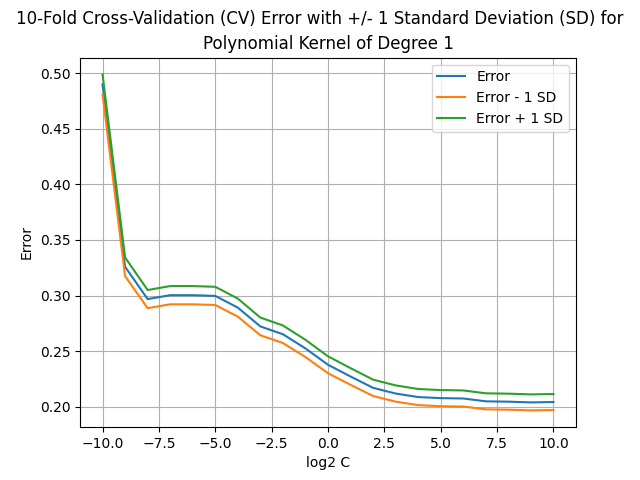
\includegraphics[width=.45\textwidth]{graphics/hw2/4.1.png}
            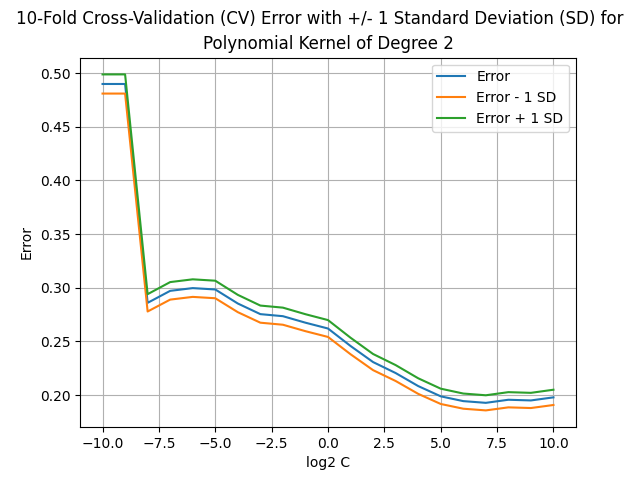
\includegraphics[width=.45\textwidth]{graphics/hw2/4.2.png}
            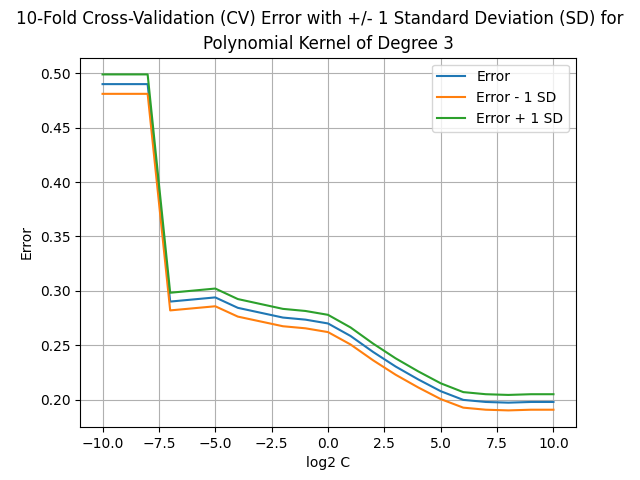
\includegraphics[width=.45\textwidth]{graphics/hw2/4.3.png}
            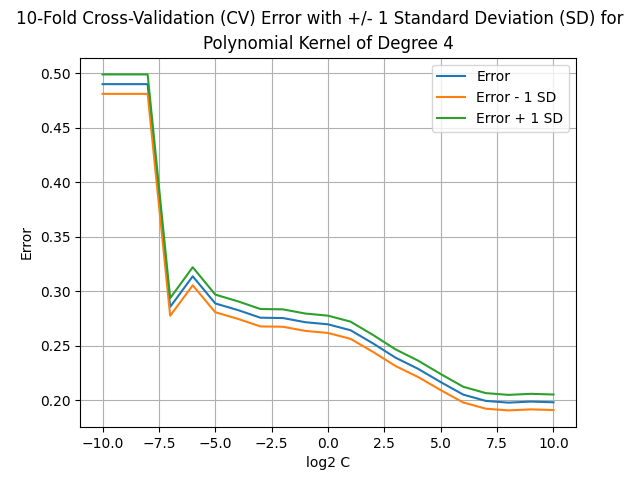
\includegraphics[width=.45\textwidth]{graphics/hw2/4.4.png}
        \end{center}
        \caption{10-fold cross-validation error of SVM with polynomial
        kernels and degree $d=1,2,3,4$ (going clockwise) plotted with
        standard deviation by values of $\log_2 C$.}
        \label{fig:4}
    \end{figure}

    \item For large $\log_2 C$, the errors are nearly indistinguishable.
    However, we achieve one of the lowest errors when $d^*=2$ and $C^*=128$.
    We set $C=128$ and use $d=1,\ldots,6$.
    We extract the accuracy again with scriptextract.py and count support vectors
    with  scriptcount.py (\autoref{lst:scriptcount}).
    We plot the testing error in \autoref{fig:5error}
    and number of support vectors in \autoref{fig:5supports}
    using scriptplot5.py (\autoref{lst:scriptplot5}).
    \begin{figure}[ht]
        \begin{center}
            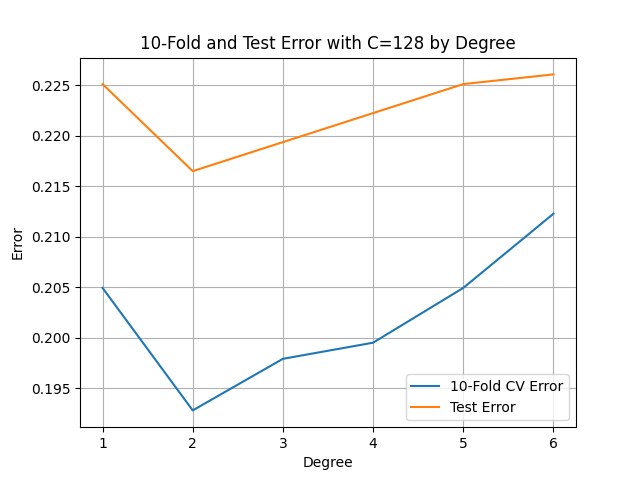
\includegraphics[width=.45\textwidth]{graphics/hw2/5error.png}
        \end{center}
        \caption{Error on 10-fold cross-validation and
        testing data as a function of degree.}
        \label{fig:5error}
    \end{figure}
    \begin{figure}[ht]
        \begin{center}
            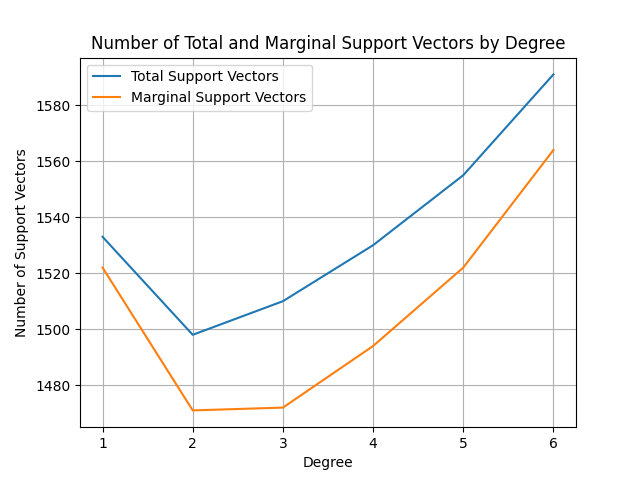
\includegraphics[width=.45\textwidth]{graphics/hw2/5supports.png}
        \end{center}
        \caption{Number of total and marginal support vectors
        as a function of degree.}
        \label{fig:5supports}
    \end{figure}

    \autoref{fig:5error} shows that the test error decreases and then
    increases with $d$.
    The error on the testing data is slightly higher than the 10-fold
    cross-validation error.
    \autoref{fig:5supports} shows that the number of total and marginal
    support vectors decreases and then increases with $d$.
 
    \item 
    The use of $\alpha$ as a coefficient in the book
    is difficult to reconcile with $\alpha$ as a sparsity vector.
    \textcolor{red}{
    Therefore we denote the sparsity vector by $a$
    and the coefficients by $\alpha'$, $\beta'$, and $\gamma'$.}
    With this notation, the optimization problem is
    \begin{align}\label{eq:primal}
        \min_{a,b} \frac{1}{2}\sum_{i=1}^m a_i^2
        + C\sum_{i=1}^m \xi_i
    \end{align}
    subject to the constraints that
    \begin{align}\label{eq:ourconstraint}
        y_i\left(
        \sum_{j=1}^m a_i y_j K(x_i,x_j)
        +b \right) \geq 1 - \xi_i
    \end{align}
    and $\xi_i,a_i\geq 0$ for $i \in [m]$.
    \begin{enumerate}
        \item The general primal optimization problem is
        equivalent to the above optimization problem except for
        the first constraint (and the non-negativity constraint
        on $a$) which, in the primal optimization problem of SVMs, is
        \begin{align}\label{eq:theirconstraint}
            y_i(a\cdot z_i + b) \geq 1 - \xi_i.
        \end{align}
        We show that, modulo the non-negativity constraint on $a$,
        the problem coincides with an instance of
        the primal optimization by constructing $z_i$
        such that \autoref{eq:ourconstraint} and
        \autoref{eq:theirconstraint} are equivalent.
        Let $z_i$ be a vector whose $j$th entry for
        $j\in[m]$ is $y_j(x_j\cdot x_i)$.
        Then
        \begin{align}
            y_i(a \cdot z_i + b) =
            y_i\left(
            \sum_{j=1}^m a_i y_j (x_i \cdot x_j)
            +b \right) = 
            y_i\left(
            \sum_{j=1}^m a_i y_j K(x_i,x_j)
            +b \right)
            \nonumber
        \end{align}
        where $K(x_i,x_j)$ is the dot product.
        Then clearly the given optimization problem and
        the following primal optimization problem of SVMs
        are equivalent:
        \begin{align}
            \min_{a,b} \frac{1}{2}\sum_{i=1}^m a_i^2
            + C\sum_{i=1}^m \xi_i
            \nonumber
        \end{align}
        subject to the constraints that
        \begin{align}
            y_i(a\cdot z_i + b)\geq 1 - \xi_i
            \nonumber
        \end{align}
        and $\xi_i\geq 0$ for $i \in [m]$
        (sans the non-negativity constraint on $a$).

        \item We answer this question by referencing
        the dual optimization problem we derive in the next question.
        The objective function of the dual is
        $G: a \rightarrow 
        -\frac{1}{2} \sum_{k=1}^m\sum_{l=1}^m \alpha_k'
        \alpha_l' y_k y_l K(x_k,x_l)
        + \frac{1}{2} \sum_{i=1}^m \gamma_i'^2
        + \sum_{i=1}^m\alpha_i'$.
        $G$ is infinitely differentiable.
        Its Hessian is given by $\nabla^2G=-K$.
        For the problem to be a convex optimization problem,
        we need $\nabla^2G$ to be concave.
        That is, $\nabla^2G \preceq 0$.
        Luckily we have this when $K$ is positive definite symmetric
        (PDS) since then $K \succeq 0$ and $-K \preceq 0$ as required.
        Therefore we need the condition that $K$ is PDS
        for \autoref{eq:primal} to be a convex optimization problem.

        \item \textcolor{red}{Important: to reconcile the notation of
        the book and problem, we use $a$ to represent the
        sparsity vector we want to minimize and $\alpha_i'$,
        $\beta_i'$ and $\gamma_i'$ to represent coefficients
        in the optimization problem.}

        The Lagrangian is
        \begin{align}
            L(a, b, \xi, \alpha', \beta', \gamma')
            &= \frac{1}{2}{\norm{a}^2} + C \sum_{i=1}^m\xi_i
            - \sum_{i=1}^m\alpha_i'(y_i(\sum_{j=1}^m a_j y_j x_j
            \cdot x_i + b)-1 + \xi_i) \nonumber \\
            &- \sum_{i=1}^m\beta_i'\xi_i - \sum_{i=1}^m\gamma_i'a_i
            \nonumber \\
            &= \frac{1}{2}{\norm{a}^2} + C \sum_{i=1}^m\xi_i
            - (\sum_{i=1}^m\alpha_i'y_i x_i)
            (\sum_{j=1}^m a_j y_j x_j) \nonumber \\
            &- \sum_{i=1}^m\alpha_i'y_i b + \sum_{i=1}^m\alpha_i'
            - \sum_{i=1}^m\alpha_i'\xi_i
            - \sum_{i=1}^m\beta_i'\xi_i - \sum_{i=1}^m\gamma_i'a_i.
            \nonumber
        \end{align}
        Then the KKT conditions yield
        \begin{align}
            \nabla_{a_i}L &= a_i - y_i x_i \sum_{k=1}^m
            \alpha_k'y_k x_k - \gamma_i' = 0
            \label{eq:kkta} \\
            \nabla_{b}L &= -\sum_{i=1}^m\alpha_i' y_i = 0
            \label{eq:kktb} \\
            \nabla_{\xi_i}L &= C - \alpha_i' - \beta_i' = 0
            \label{eq:kktxi}
        \end{align}
        subject to the constraints that
        \begin{align}
            \alpha_i'(y_i(\sum_{j=1}^m a_j y_j x_j\cdot x_i
            + b) -1 +\xi_i) 
            =\beta_i'x_i
            =\gamma_i'a_i=0
            \nonumber
        \end{align}
        for $i \in [m]$.
        Now we simplify the Lagrangian with the
        new information:
        \begin{align}
            L &= \frac{1}{2}\norm{a}^2 + C\sum_{i=1}^m
            - \sum_{i=1}^m a_i(a_i-\gamma_i')
            - b\sum_{i=1}^m\alpha_i'y_i \nonumber \\
            &+ \sum_{i=1}^m\alpha_i' -\sum_{i=1}^m \alpha_i' \xi_i
            - \sum_{i=1}^m\beta_i' \xi_i - \sum_{i=1}^m a_i \gamma_i'.
            \nonumber
        \end{align}
        We use the following expressions:
        $y_i x_i \sum_{k=1}^m \alpha_k'y_k x_k = a_i -\gamma_i'$
        from \autoref{eq:kkta},
        $\alpha_i'+\beta_i'=C$ from \autoref{eq:kktb}, and
        $\sum_{i=1}^m \alpha_i'y_i=0$ from \autoref{eq:kktxi}.
        Then we simply have
        \begin{align}
            L=-\frac{1}{2}\norm{a}^2 + \sum_{i=1}^m \alpha_i'.
            \nonumber
        \end{align}
        Unfortunately $\norm{a}^2$ is not so simple:
        \begin{align}
            \norm{a}^2 &= \sum_{i=1}^m(y_i x_i
            \sum_{k=1}^m \alpha_k' y_k x_k +\gamma_i')^2
            \nonumber \\
            &= \sum_{i=1}^m [(y_i x_i \sum_{k=1}^m \alpha_k' y_k x_k)^2
            + \gamma_i'^2 + 2\gamma_i y_i x_i \sum_{k=1}^m \alpha_k' y_k x_k].
            \nonumber
        \end{align}
        Here, we get lucky since we know $\gamma_i'a_i = 0$
        from the constraints on the KKT conditions so
        $\gamma_i'(y_i x_i \sum_{k=1}^m \alpha_k' y_k x_k +\gamma_i')=0$
        and
        $\gamma_i'^2 = -\gamma_i'y_i x_i \sum_{k=1}^m \alpha_k' y_k x_k$.
        Then 
        \begin{align}
            &= \sum_{i=1}^m[y_i^2 x_i^2 \sum_{k=1}^m\alpha_k'y_k x_k
            \sum_{l=1}^m\alpha_l'y_l x_l + \gamma_i'^2 - 2\gamma_i'^2]
            \nonumber \\
            &= \sum_{k=1}^m\sum_{l=1}^m \alpha_k'\alpha_l' y_k y_l
            \sum_{i=1}^m(x_i y_i x_k) (x_i y_i x_l)
            - \sum_{i=1}^m \gamma_i'^2 \nonumber \\
            &= \sum_{k=1}^m\sum_{l=1}^m \alpha_k'\alpha_l' y_k y_l K(x_k,x_l)
            - \sum_{i=1}^m \gamma_i'^2 \nonumber.
        \end{align}
        We combine our expression for $\norm{a}^2$ with 
        our expression for $L$.
        We have that the dual optimization problem is
        \begin{align}
            \max_{\alpha', \gamma'}
            -\frac{1}{2} \sum_{k=1}^m\sum_{l=1}^m \alpha_k'\alpha_l' y_k y_l K(x_k,x_l)
            + \frac{1}{2} \sum_{i=1}^m \gamma_i'^2
            + \sum_{i=1}^m\alpha_i'
            \nonumber
        \end{align}
        subject to the constraints that $0 \leq \alpha_i' \leq C$
        (since $\beta_i'\geq0$ and $\beta_i'+\alpha_i'=C$) and
        $\sum_{i=1}^m\alpha_i'y_i=0$ for $i \in [m]$.
        (Clearly any real $\gamma_i'$ suffices because then
        $\gamma_i'^2$ has to be non-negative which is what we need.)

        \item We transform the data into the sparsity minimization problem
        using the $z_i$ constraint transformation in \autoref{eq:theirconstraint}
        via scriptpreprocess6.py (\autoref{lst:preprocess6}).
        We then scale the data, making sure to use the range of the training
        data for both the training and test data.
        Next, we identify good values of $C$.
        Again, the error becomes almost indistinguishable but one of the best
        values is $C^*=32$.
        We then calculate the error
        rates of 10-fold cross-validation and the test data.
        We plot the data with scriptplot6.py (\autoref{lst:scriptplot6}).
        \autoref{fig:6error} shows the error of the 10-fold cross-validation
        roughly increases with $d$ while the error on the testing data
        roughly decreases.
        The errors are approximately the same for $d\leq3$ but for $d\geq4$ the
        test error is surprisingly smaller.
        The whole approach can be found in script6.sh (\autoref{lst:script6}).
        \begin{figure}[ht]
            \begin{center}
                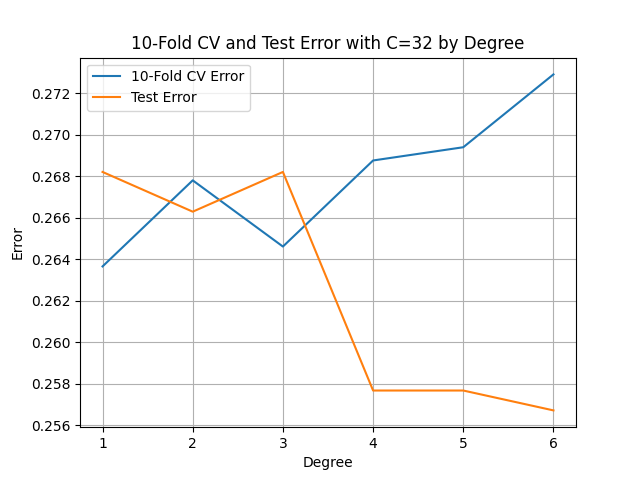
\includegraphics[width=.45\textwidth]{graphics/hw2/6error.png}
            \end{center}
            \caption{Error on 10-fold cross-validation and
            testing data as a function of degree.}
            \label{fig:6error}
        \end{figure} 


    \end{enumerate}
\end{enumerate}

\appendix
\section*{Appendix}
\lstinputlisting[label={lst:script3}, language=Bash, caption={Scaling training data and then using training range to scale test data.}]{code/hw2/script3.sh}
\lstinputlisting[label={lst:preprocess3}, language=Python, caption={Preprocessing abalone.data.}]{code/hw2/scriptpreprocess3.py}
\lstinputlisting[label={lst:script4}, language=Bash, caption={Finding good $d$ and $C$ parameters via 10-fold cross-validation accuracy.}]{code/hw2/script4.sh}
\lstinputlisting[label={lst:scriptextract}, language=Python, caption={Extract accuracy parameter.}]{code/hw2/scriptextract.py}
\lstinputlisting[label={lst:scriptplot4}, language=Python, caption={Plot error rate as a function of $\log_2 C$.}]{code/hw2/scriptplot4.py}
\lstinputlisting[label={lst:script5}, language=Bash, caption={Error rate on 10-fold cross-validation and testing in addition to number of total and marginal support vectors.}]{code/hw2/script5.sh}
\lstinputlisting[label={lst:scriptcount}, language=Python, caption={Count the number of total and marginal support vectors.}]{code/hw2/scriptcount.py}
\lstinputlisting[label={lst:scriptplot5}, language=Python, caption={Plot error of 10-fold cross-validation and testing data as well as total and marginal support vectors by degree.}]{code/hw2/scriptplot5.py}
\lstinputlisting[label={lst:script6}, language=Bash, caption={Scaling data, finding a good $C$, and finding and plotting error.}]{code/hw2/script6.sh}
\lstinputlisting[label={lst:preprocess6}, language=Python, caption={Transform data into sparsity minimization problem.}]{code/hw2/scriptpreprocess6.py}
\lstinputlisting[label={lst:scriptplot6}, language=Python, caption={Plot error of 10-fold cross-validation and testing data.}]{code/hw2/scriptplot6.py}



\homework{3}{R. Teal Witter}
% chktex-file 46
% chktex-file 3
% chktex-file 24

\section*{A. Kernel Methods}
\medskip

\begin{enumerate}
    \item Let $W = (W_{p,q})$ be a symmetric
    $n \times n$ matrix
    where $W_{p,q}$ is the weight of the edge between
    nodes $p$ and $q$ and $n$ is the number of nodes
    in the graph.
    Observe that $W_{p,q}$ if there is no edge between
    $p$ and $q$.
    Now consider the matrix $K = W^T W$.
    An entry $K(p,q)$ is
    \begin{align} \label{eq:weights}
        \sum_{u \in V} W_{p,u}^T W_{u,q}.
    \end{align}
    Observe that \autoref{eq:weights} is exactly
    the sum of the weights
    of all paths of length two between $p$ and $q$:
    If $u$ is not on a path of length two between $p$ and $q$,
    then either $u$ does not share an edge with $p$
    or with $q$ and so $u$ contributes 0 to the sum.
    If $u$  is on a path of length two between $p$ and $q$,
    then there is an edge between $p$ and $u$ and $u$ and $q$
    and so $u$ contributes the product of the weights to the sum.

    Now we want to show that $K$ is PDS.
    Let $\mathbf{c} \in \R^{n\times 1}$.
    Then
    \begin{align}
        \mathbf{c}^T W^T W \mathbf{c}
        = ||W \mathbf{c}||_2^2 \geq 0.
        \nonumber
    \end{align}
    Therefore $K$ is a PDS kernel.

    \item Pixel kernel
    \begin{enumerate}
    \item Note that
    \begin{align}
        \int_{t=0}^\infty 1_{t \in [0,z]} 1_{t \in [0,z']} dt
        = \langle 1_{[0,z]}, 1_{[0,z']} \rangle.
        \nonumber
    \end{align}
    When $z$ or $z'$ is negative, then $S$ returns 0
    since $t \notin [0,z], [0,z']$ when $t\geq 0$.
    Otherwise, $S(z,z') = \min\{z, z'\}$
    since we only have non-zero values when
    $0 \leq t \leq z,z'$.

    To show that $S$ is PDS, let $\mathbf{c}$
    be any real vector.
    Then
    \begin{align}
        \langle \mathbf{c} 1_{[0,z]}, \mathbf{c} 1_{[0,z']}
        \rangle
        = ||c||_2^2 \langle 1_{[0,z]}, 1_{[0,z']} \rangle
        \geq 0
        \nonumber
    \end{align}
    since every element in $1_{[0,z]}$ and $1_{[0,z']}$
    is nonnegative.
    Therefore $S$ is a PDS kernel.

    \item Fix $k \in [N]$.
    From (a), we know that 
    $\min \{|x_k|^\mu, |x_k'|^\mu \}
    = S(|x_k|^\mu, |x_k'|^\mu)$.
    (Since $|x_k|^\mu$ and $|x_k'|^\mu$ 
    are both positive, we don't
    have to worry about negative values.)

    Then $\exp(\min \{|x_k|^\mu, |x_k'|^\mu \})$
    is also PDS
    from Theorem 6.10 (PDS kernels - closure properties)
    in the book.
    That is, composition with a power series
    with non-negative coefficients (i.e. $\exp$)
    preserves the PDS property.

    The final step is to take the product of
    $\exp(\min \{|x_k|^\mu, |x_k'|^\mu \})$
    over $k \in [N]$.
    The product of two PDS kernels
    is also PDS (again by Theorem 6.10).
    By repeated application of this property,
    we can extend it to the product of
    any finite number of PDS kernels.

    Therefore
    \begin{align}
        \prod_{k=1}^N
        e^{\min \{|x_k|^\mu, |x_k'|^\mu \}}
        \nonumber
    \end{align}
    is PDS.
    \end{enumerate}
\end{enumerate}

\subsection*{B. Boosting}

\begin{enumerate}
\item Logistic loss boosting
\begin{enumerate}
    \item To show that $\Phi$ is convex we show that
    its second derivative is positive for
    $u \in \textrm{dom}(\Phi)$
    and $\textrm{dom}(\Phi)$ is a convex set.
    The domain of $\Phi$ is the set of real numbers $\R$.
    The set of real numbers is clearly convex:
    for $x, y \in \R$, any number between $x$ and $y$
    must also be in $\R$.
    We take the derivatives of $\Phi$:
    \begin{align}
        \Phi(u) &= \log_2(1+e^{-u}) \nonumber \\
        \Phi'(u) &= \frac{1}{\ln(2)}\frac{-e^{-u}}{1+e^{-u}}
        \nonumber \\
        \Phi''(u) &= -\frac{1}{\ln(2)}\frac
        {-(1+e^{-u})e^{-u} - e^{-u}e^{-u}}
        {(1+e^{-u})^2} = \frac{1}{\ln(2)}
        \frac{1}{(1+e^{u})^2} \geq 0
        \nonumber
    \end{align}
    for all $u \in \R$.
    Therefore $\Phi$ is convex.

    To see that $\Phi$ is decreasing,
    take $x<y$ for $x,y \in \R$.
    Then
    \begin{align}
        -x > -y &\Leftrightarrow
        e^{-x} > e^{-y} \nonumber \\
        &\Leftrightarrow
        1+e^{-x} > 1+e^{-y} \nonumber \\
        &\Leftrightarrow
        \log_2(1+e^{-x}) > \log_2(1+e^{-y})
        \nonumber \\
        &\Leftrightarrow
        \Phi(x) > \Phi(y)
        \nonumber
    \end{align}
    since both $\log_2$ and $\exp$ are monotone
    increasing.
    Therfore $\Phi$ is decreasing.

    To see that $\Phi$ upper bounds the
    zero-one loss, take $0\geq x$.
    Then
    \begin{align}
        0 \leq - x &\Leftrightarrow
        e^0 = 1 \leq e^{-x} \nonumber \\
        &\Leftrightarrow
        \log_2(1 + 1) \leq \log_2(1+e^{-x}) \nonumber \\
        &\Leftrightarrow
        1 \leq \Phi(x).
        \nonumber
    \end{align}
    Now take $0\leq x$,
    \begin{align}
        e^{-x} \geq 0 &\Leftrightarrow
        1 + e^{-x} \geq 1 \nonumber \\
        &\Leftrightarrow
        \log_2(1+e^{-x}) \geq 0 \nonumber \\
        &\Leftrightarrow
        \Phi(x) \geq 0
        \nonumber
    \end{align}
    where the the first inequality
    follows from the positivity of $e^{y}$
    for all $y\in \R$.
    Together, $\Phi(x) \geq 1$ when $x$ is negative
    (i.e. the zero-one loss ``fires'')
    and $\Phi(x) \geq 0$ when $x$ is positive
    (i.e. the zero-one loss stays at 0).
    Thefore $\Phi$ upperbounds the zero-one loss.

    \item
    Let the function
    $f(x) = \sum_{j=1}^N \alpha_j h_j (x)$
    for a given $N$-length vector of
    non-negative coefficients $\alpha$
    where $h_j$ is in the hypothesis set $H$ and $H$
    has cardinality $N$.
    For pairs of points and labels $(x_i, y_i)$ where $i \in [m]$,
    define the objective function
    \begin{align}
        F(\alpha) = \frac{1}{m} \sum_{i=1}^m
        \log_2(1+e^{-y_i\sum_{j=1}^p\alpha_j h_j (x_i)}).
        \nonumber
    \end{align}

    We now argue that $F$ is convex with respect to $\alpha$:
    $-y_i f(x_i)$ is convex
    because it is an affine function of $\alpha$.
    $\Phi$ is convex by (a) and so
    $\log_2(1+\exp(-y_i f(x_i)))$ is also convex
    since composition with a monotone increasing
    convex function (i.e. $\Phi$) preserves convexity.
    Finally the sum of convex functions is convex and multiplying
    by a scalar does not affect convexity.
    Therefore $F$ is convex with respect to $\alpha$.

    \item
    For $t \in [T]$ and $k \in [N]$, define
    \begin{align}
        f_t &= \sum_{j=1}^N \alpha_t h_j(x_i) \nonumber \\
        Z_t &= \sum_{i=1}^m \frac{e^{-y_i f_{t-1}(x_i)}}
        {\ln(2)(1+e^{-y_i f_{t-1}(x_i)})} \nonumber \\
        D_t(i) &= \frac{e^{-y_i f_{t-1}(x_i)}}
        {\ln(2)(1+e^{-y_i f_{t-1}(x_i)})Z_t} \nonumber \\
        \epsilon_{t,k} &= \E_{i \sim D_t}
        [1_{y_i h_k(x_i)} \leq 0].
        \nonumber
    \end{align}

    The directional derivative of $F$ at $\alpha_{t-1}$
    along $e_k$ is defined by
    \begin{align}
        F'(\alpha_{t-1},e_k) &= \lim_{\eta \rightarrow 0}
        \frac{F(\alpha_{t-1}, e_k) - F(\alpha_{t-1})}
        {\eta} 
        \textrm{ where} \nonumber \\
        F(\alpha_{t-1}, \eta e_k) &= \frac{1}{m}
        \sum_{i=1}^m \log_2(1+e^{-y_i \sum_{j=1}^N
        \alpha_{t-1}h_j(x_i) - \eta y_i h_k(x_i)}).
        \nonumber
    \end{align}
    Then taking the derivative with respect to $\eta$
    and immediately setting $\eta$ to 0 yields
    \begin{align}
        F'(\alpha_{t-1}, e_k) &=
        -\frac{1}{m} \sum_{i=1}^m
        \frac{y_i h_k(x_i) e^{-y_i f_{t-1}(x_i)}}
        {\ln(2)(1+e^{-y_i f_{t-1}(x_i)})} \nonumber \\
        &= -\frac{1}{m} \sum_{i=1}^m y_i h_k(x_i)
        D_t Z_t \nonumber \\
        &= -\frac{Z_t}{m} \left [
        \sum_{i=1}^m D_t(i) 1_{y_i h_k(x_i)=1}
        - \sum_{i=1}^m D_t(i) 1_{y_i h_k(x_i)=-1}
        \right] \nonumber \\
        &= -\frac{Z_t}{m} \left [
        (1-\epsilon_{e,k}) - \epsilon_{e_k}
        \right]
        = \frac{Z_t}{m} \left [
        2 \epsilon_{t,k} - 1
        \right ].
        \label{eq:max}
    \end{align}
    We want to maximize the absolute value
    of \autoref{eq:max} to get the best descent
    so we want the smallest value of $\epsilon_{t,k}$
    (since $Z_t$ and $m$ do not change with respect
    to the choice of $k$).
    Therefore when boosting on the $t$th iteration
    we want to find $k$ such that $\epsilon_{t,k}$
    is smallest.
    Observe that our weak learning condition must be
    that there is some $k$ such that
    $\epsilon_{t,k} \leq 1/2$ on the $t$th iteration,
    for the distribution $D_t$, and for the sample
    of $m$ points.

    \item Fix $(u,v) \in \R^2$, then
    \begin{align}
        \Phi(u+v) - \Phi(u) &= \log_2(1+e^{-u-v})
        - \log_2(1+e^{-u}) \nonumber \\
        &= \log_2 \left( \frac{1+e^{-u-v}}{1+e^{-u}}
        \right) \nonumber \\
        &= \log_2 \left( \frac{(e^{-v}-1)e^{-u} + 1+ e^{-u}}{1+e^{-u}}
        \right) \nonumber \\
        \label{eq:continuin}
        &= \log_2 \left( \frac{(e^{-v}-1)e^{-u}}{1+e^{-u}} +1
        \right).
    \end{align}
    Now define $x=(e^{-v}-1)e^{-u}/(1+e^{-u})$.
    Observe that $x\geq -1$ since $e^{-v} \geq 0$
    and $1 \geq e^{-u}/(1+e^{-u}) \geq 0$ for all $u,v \in \R$.

    We want to show that $f(x) = x - \ln(x+1) \geq 0$
    for $x \geq -1$.
    Together 
    \begin{align}
        f'(x) &= 1 - 1/(x+1)  = 0 \Leftrightarrow x = 0
        \nonumber \\ &\textrm {and} \nonumber \\
        f''(x) &= 1/(x+1)^2 > 0
        \nonumber
    \end{align}
    imply that $x=0$ is minimal point.
    Since 
    \begin{align}
        \lim_{x\rightarrow -1^+} f(x) = \infty
        = \lim_{x\rightarrow \infty} f(x)
        \nonumber
    \end{align}
    $x=0$ is indeed a global minimum.
    Then $f(0)=0$ implies that $f(x) \geq 0$ so
    \begin{align}\label{eq:lnineq}
        \ln(x+1) \leq x
    \end{align}
    for $x \geq -1$.

    Continuing from \autoref{eq:continuin},
    we use \autoref{eq:lnineq} and get that
    \begin{align}
        \Phi(u+v) - \Phi(u) &= 
        \ln \left( \frac{(e^{-v}-1)e^{-u}}{1+e^{-u}} +1
        \right) \nonumber \\
        &\leq
        \ln \left( \frac{(e^{-v}-1)e^{-u}}{1+e^{-u}} +1
        \right) 
        \frac{1}{\ln(2)} \nonumber \\
        &\leq \frac{(e^{-v}-1)e^{-u}}{\ln(2)(1+e^{-u})}
        \nonumber \\
        &= -\frac{-e^{-u}}{\ln(2)(1+e^{-u})}(e^{-v}-1)
        = -\Phi'(u) (e^{-v}-1).
        \nonumber
    \end{align}
    Therefore
    \begin{align}\label{eq:phiinequal}
        \Phi(u+v) - \Phi(u)
        \leq -\Phi'(u) (e^{-v}-1)
    \end{align}
    for all $(u,v) \in \R^2$.

    \item
    We have
    \begin{align}
        F(\alpha_{t-1} + \eta e_k) - F(\alpha_{t-1})
        &= \frac{1}{m} \sum_{i=1}^m \log_2
        (1+e^{-y_i \sum_{j=1}^N \alpha_{t-1, j} h_j(x_i)
        -\eta y_i h_k(x_i)})
        \nonumber \\
        &- \frac{1}{m} \sum_{i=1}^m \log_2
        (1+e^{-y_i \sum_{j=1}^N \alpha_{t-1, j} h_j(x_i)})
        \nonumber.
    \end{align}
    Define $u_i = y_i \sum_{j=1}^N \alpha_{t-1, j} h_j(x_i)$
    and $v_i = \eta y_i h_k(x_i)$.
    Then using \autoref{eq:phiinequal}
    \begin{align}
        F(\alpha_{t-1} + \eta e_k) - F(\alpha_{t-1})
        &= \frac{1}{m} \sum_{i=1}^m
        \Phi(u_i + v_i) - \Phi(u_i) \nonumber \\
        &\leq \frac{1}{m} \sum_{i=1}^m
        - \Phi'(u_i) (e^{-v_i}-1) \nonumber \\
        &= \frac{1}{m} \sum_{i=1}^m
        -\frac{-e^{-u_i}}{\ln(2)(1+e^{u_i})}
        (e^{-v_i}-1) \nonumber \\
        &= \frac{1}{m} \sum_{i=1}^m
        D_t(i) Z_t (e^{-\eta y_i h_k(x_i)}-1).
        \nonumber
    \end{align}
    Therefore
    \begin{align}\label{eq:Finequality}
        F(\alpha_{t-1} + \eta e_k) - F(\alpha_{t-1})
        \leq \frac{1}{m} \sum_{i=1}^m
        D_t(i) Z_t (e^{-\eta y_i h_k(x_i)}-1).
    \end{align}

    \item
    We minimize the upper bound in \autoref{eq:Finequality}
    by differentiating with respect to $\eta$ and
    setting the result equal to 0.
    We get
    \begin{align}
        \frac{1}{m} \sum_{i=1}^m D_t(i)Z_t
        (-y_i h_k(x_i) e^{-\eta y_i h_k(x_i)}) &= 0
        \nonumber \\
        -\frac{Z_t}{m} \left[
        \sum_{i=1}^m D_t(i) 1_{y_i h_k(x_i) = 1} e^{-\eta}
        - \sum_{i=1}^m D_t(i) 1_{y_i h_k(x_i) = -1} e^{\eta}
        \right] &= 0 \nonumber \\
        (1-\epsilon_{t,k})e^{-\eta} - \epsilon_{t,k} e^\eta &= 0
        \nonumber \\
        \frac{1-\epsilon_{t,k}}{\epsilon_{t,k}} &= e^{2\eta}
        \nonumber \\
        \frac{1}{2} \ln \left(
        \frac{1-\epsilon_{t,k}}{\epsilon_{t,k}} \right)
        &= \eta.
        \label{eq:stepsize}
    \end{align}
    \autoref{eq:stepsize} is exactly the same as the minimization
    step size (there the variable is $\alpha_t$) in AdaBoost
    since our $\epsilon_{t,k}$ is their $\epsilon_t$.
    (Their $\epsilon_t$ is defined to be in the best direction $k$.)

    At iteration $t$, the step is given by
    $\alpha_t = \alpha_{t-1} + \eta e_k$
    where $\eta$ is the step size given in 
    \autoref{eq:stepsize} and $e_k$ is the step direction
    chosen because its error is smallest.
    In terms of $f_t = \sum_{i=j}^N \alpha_{t,j} h_j$,
    the step is given by
    $f_t = f_{t-1} + \eta h_k = f_{t-1} + \alpha_t h_t$
    where $\alpha_t = \eta$ and $h_t=h_k$ are alternate
    notation for the step size and direction.

    \item The pseudocode appears in \autoref{lst:logreg}.

    \begin{minipage}{\linewidth}
    \begin{lstlisting}[caption={Logistic loss boosting.}, label={lst:logreg}]
  input: set of samples $S= ((x_1,y_1),\ldots, (x_m, y_m))$,
         number of iterations $T$,
         hypothesis set $H$ with $N$ base predictors
  output: function $f$
  $f_0 \gets 0$
  for $i \gets 1$ to $m$ do
    $D_1(i) \gets 1/m$
  for $t \gets 1$ to $T$ do
    $h_t \gets \arg \min_{h \in H} \Pr_{i \sim D_t}(h(x_i) \neq y_i)$
    $\epsilon_t \gets \Pr_{i \sim D_t}(h_t(x_i) \neq y_i)$
    $\alpha_t \gets \frac{1}{2} \ln(\frac{1-\epsilon_{t}}{\epsilon_{t}})$
    $f_t \gets f_{t-1} + \alpha_t h_t$
    $Z_{t+1} \gets \sum_{i=1}^m e^{-y_i f_{t}(x_i)}/(\ln(2)(1+e^{-y_i f_{t}(x_i)}))$
    for $i \gets 1$ to $m$ do
      $D_{t+1}(i) \gets e^{-y_i f_{t}(x_i)}/(\ln(2)(1+e^{-y_i f_{t}(x_i)})Z_{t+1})$
  return $f_T$
    \end{lstlisting}
    \end{minipage}

    \item
    We will use Corollary 7.5 and Corollary 7.6 from the book.
    They cannot be directly applied to the function returned
    from \autoref{lst:logreg} since it is not a convex combination
    of base hypotheses.
    Instead, define
    $\bar{f} = \sum_{t=1}^T \alpha_t h_t / (||\alpha||_1) \in \textrm{conv}(H)$
    where $\alpha$ is the vector with 0 entries in the positions corresponding
    to $h$ that are not picked in any iteration $t \in [T]$ and $\alpha_t$
    in the positions corresponding to $h_t$ that are picked at iteration $t$.
    Observe that $\bar{f}$ and $f$ are equivalent in the context
    of binary classification since $\textrm{sgn}(f) = \textrm{sgn}(f/||\alpha||_1)$.
    It follows that $R(f) = R(f/||\alpha||_1)$.

    Then for $H$ a set of real-valued functions, margin $\rho>0$, any
    $\delta>0$, and $\bar{f} \in \textrm{conv}(H)$,
    Corollary 7.5 (Ensemble Rademacher margin bound) yields
    \begin{align}
        R(f) = R(\bar{f}) \leq \hat{R}_{S,\rho}(\bar{f}) + \frac{2}{\rho}
        \mathcal{R}_m(H) + \sqrt{\frac{\ln(1/\delta)}{2m}}
        \nonumber
    \end{align}
    with probability $1-\delta$.

    We also have the option to bound the Rademacher complexity like so
    \begin{align}
        \mathcal{R}_m(H) \leq \sqrt{\frac{2d\log(em/d)}{m}}
        \nonumber
    \end{align}
    as in Corollary 7.6 (Ensemble VC-Dimension margin bound).

    Define
    \begin{align}
        \rho_f = \min_{i\in[m]} \frac{|\alpha \cdot f(x_i)|}{||\alpha||_1}.
        \nonumber
    \end{align}
    Then, since the margin loss can be upper bounded by the fraction
    of points $x$ labeled with $y$ in the training sample with confidence
    margin at most $\rho$,
    we can write
    \begin{align}
        \hat{R}_{S,\rho}(\bar{f}) \leq
        \frac{|\{i\in[m]:y_i \rho_f(x_i) \leq \rho\}|}
        {m}.
        \nonumber
    \end{align}
    Since $\Phi:u \rightarrow \log_2(1+e^{-u})$
    upper bounds the zero-one loss by part (a),
    we can also write
    \begin{align}
        \hat{R}_{S,\rho}(\bar{f})
        &= \frac{1}{m}\sum_{i=1}^m
        1_{y_i f(x_i) - \rho ||\alpha||_1 \leq 0}
        \nonumber \\
        &\leq \frac{1}{m}\sum_{i=1}^m
        \log_2(1+e^{-y_i f(x_i)+\rho||\alpha||_1}).
        \nonumber
    \end{align}

    \item

\end{enumerate}
\end{enumerate}


	
\end{document}